\chapter{Estudios del Cotransportador vSGLT}\label{ch:vSGLT}
\section{Principios de Bioqu\'{i}mica}
El presente estudio se ocupa de una prote\'{i}na encontrada en la membrana de la bacteria \textit{Vibrio Parahaemoliticus}. Pero antes de realizar dicho estudio es necesario responder las siguientes preguntas fundamentales: ?`qu\'{e} es una prote\'{i}na? ?`de qu\'{e} est\'{a} conformada una prote\'{i}na? ?`d\'{o}nde se encuentran las prote\'{i}nas? ?`cu\'{a}l es el papel que desempe\~{n}an las prote\'{i}nas en los seres vivos? ?`Cu\'{a}l es la forma de las prote\'{i}nas?.\\ \\

Una prote\'{i}na es un pol\'{i}mero (pol\'{i}- Muchas -mero: Partes) que est\'{a} formado por una gran cantidad de unidades del mismo tipo, estas unidades se conocen como amino\'{a}cidos. Espec\'{i}ficamente se dice que las prote\'{i}nas son polip\'{e}ptidos \footnote{P\'{e}ptido: Mol\'{e}cula formada por una cadena de varios amino\'{a}cidos mediante un enlace llamado pept\'{i}dico; normalmente se le dice pept\'{i}do a una cadena con menos de $20\sim30$  amino\'{a}cidos} que tienen m\'{a}s de 50 amino\'{a}cidos, haciendo que su peso molecular sea mayor a 5000 Da \cite{Kuchel}.\\

Un amino\'{a}cido es una mol\'{e}cula org\'{a}nica formada por un carbono llamado $\alpha$ alrededor del cual se encuentran los grupos funcionales carboxilo y amino, adem\'{a}s de un hidr\'{o}geno y un radical que le da la identidad a cada amino\'{a}cido, ver figura \ref{fig:amino}.\\
\begin{figure}[H]
\centering
\chemfig{C^{\alpha}(-[:0]H)(-[:90]COO^{-})(-[:180]NH_{3}^{+})(-[:270]R)}
\caption{Forma general de un L-amino\'{a}cido a pH 7. El radical \ce{R} cambia para cada amino\'{a}cido.}\label{fig:amino}
\end{figure}
A continuaci\'{o}n se muestran los 20 amino\'{a}cidos comunes \footnote{Son los incorporados en la s\'{i}ntesis de prote\'{i}nas durante la traducci\'{o}n en el ribosoma}  clasificados de acuerdo a la carga, la polaridad y la formaci\'{o}n de grupos arom\'{a}ticos. Las abreviaciones de los amino\'{a}cidos se encuentran en la secci\'{o}n Lista de S\'{i}mbolos.\\
\begin{figure}[H]
\begin{center}
\begin{picture}(100,110)
\put(0,60){\includegraphics[scale=0.3]{Kap3/nopolar.png}}
\put(70,75){\includegraphics[scale=0.3]{Kap3/aromatico.png}}
\put(0,0){\includegraphics[scale=0.3]{Kap3/polardescargado.png}}
\put(70,30){\includegraphics[scale=0.3]{Kap3/qpp.png}}
\put(70,-5){\includegraphics[scale=0.2]{Kap3/qmm.png}}
\put(0,110){No polar, grupo R alif\'{a}tico}
\put(70,110){Grupo R arom\'{a}tico}
\put(0,55){Polar descargado}
\put(70,65){Grupo R cargado positivamente}
\put(70,20){Grupo R cargado negativamente}
\end{picture}
\end{center}
\caption{Estructura de los 20 amino\'{a}cidos comunes a pH 7 clasificados seg\'{u}n su radical de color rosado. Figura tomada de \cite{Nelson2011}.}
\end{figure}
Exceptuando la glicina, todos los amino\'{a}cidos presentan la propiedad de la quiralidad, existiendo dos formas posibles para cada amino\'{a}cido: L-amino\'{a}cidos o D-amino\'{a}cidos. La distinci\'{o}n va seg\'{u}n la direcci\'{o}n en la que desv\'{i}en la luz con respecto al centro quiral que es el C-$\alpha$ del amino\'{a}cido.  Pr\'{a}cticamente todos los amino\'{a}cidos encontrados en prote\'{i}nas tienen la forma L.
\subsection{Formaci\'{o}n de P\'{e}ptidos y Prote\'{i}nas}
Dos amino\'{a}cidos reaccionan formando un enlace llamado pept\'{i}dico, esto ocurre cuando el carbono del grupo carboxilo se enlaza covalentemente con el nitr\'{o}geno del grupo amino produciendo una deshidrataci\'{o}n, es decir, liberando agua. En la figura \ref{fig:pepti} se muestran los reactantes y los productos de la reacci\'{o}n.
\begin{figure}[H]
\centering
\definesubmol\a{C^{\alpha}(-[:270]H)(-[:0]C(=[:270]O)(-[:0].\textcolor{blue}{OH}))(-[:180]NH_{2})(-[:90]R^{1})}
\definesubmol\b{C^{\alpha}(-[:270]H)(-[:0]C(=[:270]O)(-[:0]OH))(-[:180]N(-[:90]H)(-[:180].\textcolor{blue}{H}))(-[:90]R^{2})}
\definesubmol\c{C^{\alpha}(-[:90]R^{1})(-[:270]H)(-[:0]C(=[:270]O)(-[:0]N(-[:90]H)(-[:0]C^{\alpha}(-[:90]R^{2})(-[:270]H)(-[:0]COOH))))(-[:180]NH_{2})}
\schemestart
\chemfig[][scale=0.75]{!\a}\+\chemfig[][scale=0.75]{!\b}\schemestop
\schemestart\arrow{<=>[][\chemfig[scale=0.75]{H_{2}O}]} \schemestop
\chemfig[][scale=0.75]{!\c}
\caption{Formaci\'{o}n de un dip\'{e}ptido. Se muestran los reactantes sin ionizar para ejemplificar, en sus formas polii\'{o}nicas  se ioniza el amino-terminal y el carboxi-terminal}\label{fig:pepti}
\end{figure}
El enlace pept\'{i}dico es un enlace amida de la forma \ce{R^{1}C(O)NHR^{2}}. Debido a que las amidas forman una estructura de resonancia tal como se ilustra en la figura \ref{fig:amide}, el enlace pept\'{i}dico forma un enlace parcial doble. Este enlace parcial doble, como los caracter\'{i}sticos de las estructuras de resonancia, es un h\'{i}brido entre el enlace simple y el enlace doble. De hecho, Linus Pauling y Robert Corey \cite{Nelson2011}, encontraron que la longitud del enlace pept\'{i}dico era de $1.32\AA{}$ la cual es menor a la de un enlace \ce{C-N} simple ($1.49 \AA{}$) y mayor a la de un enlace doble covalente \ce{C=N} ($1.27\AA{}$). \\

\begin{figure}[H]
\centering
\definesubmol\a{-[:0,0.5]C(=[:90]\lewis{0:4:,O})(-[:0]\lewis{2:,N}(-[:270]H)(-[:0,0.5]))}
\definesubmol\b{-[:0,0.5]C(-[:90]\lewis{0:4:,O})(=[:0]\lewis{2:,N}(-[:270]H)(-[:0,0.5]))}
\definesubmol\c{-[:0,0.5]C(-[:90,,,,rddbond]O)(-[:0,,,,lddbond]N(-[:270]H)(-[:0,0.5]))}
\schemestart
\chemfig[][scale=0.75]{!\a}\arrow{<->}[0,0.75]\chemfig[][scale=0.75]{!\b}\schemestop
\schemestart\arrow{<->}[0,0.75] \schemestop
\chemfig[][scale=0.75]{!\c}
\caption{Posibles estructuras de Lewis de la ani\'{o}n amida \ce{[C(O)NH]^{-2}} que al mezclarlas producen el estado resonante.}\label{fig:amide}
\end{figure}
Otro apunte que hay resaltar es el hecho de que la distancia entre los carbonos $\alpha$ es de $3.8\AA$, \cite{Smith1996}, la cual se pone en evidencia cuando se involucra la estructura de los p\'{e}ptidos y de las prote\'{i}nas en el espacio tridimensional.

\subsection{Estructura de las Prote\'{i}nas}\label{ssec:Estruc}
De acuerdo a Kai Linderstr{\o}m-Lang, la estructura de las prote\'{i}nas puede considerarse en varios niveles, conocidos como estructuras \textit{primaria}, \textit{secundaria}, \textit{terciaria} y \textit{cuaternaria}. En lo que sigue se detallan cada uno de estos niveles.
\subsubsection{Estructura Primaria y Secundaria}
Por \textit{estructura primaria} se entiende la secuencia u orden en que se encuentran los residuos unidos por enlaces pept\'{i}dicos dentro de un p\'{e}ptido o prote\'{i}na. Generalmente se conoce primero por m\'{e}todos experimentales de clivaje, la secuencia de los residuos. Conocer la secuencia es fundamental ya que esta determina la estructura tridimensional.\\

En la figura \ref{fig:pepti} se observa un residuo contiguo al otro en forma horizontal, es decir en su estructura primaria. Sin embargo, al observar al p\'{e}ptido tridimensionalmente la cadena que se forma no es lineal. Esto se debe a interacciones no covalentes entre los \'{a}tomos que no necesariamente est\'{a}n conectados por el enlace pept\'{i}dico. Estas interacciones hacen que los grupos funcionales dentro del p\'{e}ptido se encuentren a \'{a}ngulos diferentes. Para estudiar la estructura tridimensional se describir\'{a}n inicialmente, los \'{a}ngulos de rotaci\'{o}n entre los residuos que componen al p\'{e}ptido o prote\'{i}na.\\

Linus Pauling y Robert Corey encontraron que el enlace pept\'{i}dico forma una estructura planar (r\'{i}gida) que contiene 4 \'{a}tomos enlazados alrededor del \ce{C-N}, la cual se presenta debido al enlace parcial doble, de tal manera que fija el \'{a}ngulo de rotaci\'{o}n del grupo \ce{C=O} con respecto al grupo \ce{N-H}. El \'{a}ngulo $\omega$ entre los dos grupos es, excepto cuando hay prolinas, de $180\textdegree$ (conformaci\'{o}n trans). En la figura \ref{fig:pepti2} se pueden observar los \textit{planos amida} de los residuos.\\ 
\begin{figure}[H]
\centering
\includegraphics[scale=0.3]{Kap3/peptide.png}
\caption{\'{A}ngulos dihedros $\phi$, $\psi$ y $\omega$(No mostrado). Figura tomada de \cite{Nelson2011}.}\label{fig:pepti2}
\end{figure}
El \'{a}ngulo $\phi$ es $0\textdegree$ cuando el grupo \ce{N-H} est\'{a} en la posici\'{o}n trans respecto al enlace \ce{C\alpha-C} mientras que el \'{a}ngulo $\psi$ es  $0\textdegree$ cuando el enlace \ce{C-N} est\'{a} en la posici\'{o}n trans respecto al enlace \ce{C=O}, ver \cite{Kuchel}.\\

La \textit{estructura secundaria} se define como la conformaci\'{o}n local que genera estructuras repetitivas. Al definir la estructura secundaria se simplifica el entendimiento de la estructura tridimensional de la prote\'{i}na ya que permite identificar patrones que se repiten en diferentes prote\'{i}nas.\\

Existen tres tipos com\'{u}nes de estructura secundaria, ver \cite{Kuchel}:
\begin{enumerate}
 \item $\alpha$ H\'{e}lice: Ocurre si la cadena principal se enrolla formando una h\'{e}lice, de tal manera que el ox\'{i}geno del grupo carbonilo en un residuo forma un \textit{puente de hidr\'{o}geno} con el hidr\'{o}geno de la amina secundaria encontrado 4 residuos m\'{a}s adelante. En la figura \ref{fig:helice} se observan mediante las l\'{i}neas punteadas, \'{a}tomos de ox\'{i}geno (rojo) interactuando con los protones (gris claro)  en otro residuo. La cadena principal o esqueleto se representa con una cinta enrollada, figura de la izquierda cumpliendo la propiedad de tener 3.6 residuos por cada vuelta. Se observa que la secuencia en la h\'{e}lice avanza seg\'{u}n la regla de la mano derecha, esto es caracter\'{i}co de todas las h\'{e}lices formadas por L-amino\'{a}cidos, estas se les denomina $\alpha_R$ h\'{e}lices (Dextr\'{o}giras).
 \item Hoja plegada $\beta$ o l\'{a}mina $\beta$: Las hojas plegadas beta aparecen casi formando l\'{a}minas, contrario a la $\alpha$ h\'{e}lice. La hoja es formada por dos o m\'{a}s segmentos polipept\'{i}dos, contrario a la $\alpha$ h\'{e}lice, donde s\'{o}lo se requiere una cadena polipept\'{i}dica para formar la h\'{e}lice. Estos segmentos polipept\'{i}dicos est\'{a}n unidos por puentes de hidr\'{o}geno en los grupos carbonilo y amina de sus residuos. Hay dos tipos de l\'{a}minas $\beta$, las \textit{paralelas} que tienen sus cadenas polipept\'{i}dicas las mismas direccion\'{e}s, es decir del amino terminal al carboxi terminal o \textit{antiparalelas}, es decir, con direcciones opuestas entre s\'{i}. En la figura 
 \item Vueltas (Turns): Son aqu\'{e}llas conformaciones que no tienen una estructura secundaria repetitiva (pierden su estructura secundaria) e invierten la direcci\'{o}n de la cadena principal. Usualmente aparecen involucrados de 1 a 5 residuos, teniendo a estas cadenas un tama\~{n}o menor a $7\AA$. Existe una variedad de tipos de vuelta seg\'{u}n los \'{a}ngulos dihedros que formen: \cite{Pavone1996}
 \begin{enumerate}
 \item $\alpha$ Vuelta (En ingl\'{e}s $\alpha$-turn): Es com\'{u}n que sea la unidad repetitiva de una $\alpha_R$ h\'{e}lice, \cite{Pavone1996}. Se forman puentes de hidr\'{o}geno entre los grupos amino y carbonilo del primer y el quinto residuo.
 \item $\beta$ Vuelta (En ingl\'{e}s $\beta$-turn): Es la m\'{a}s com\'{u}n y se presenta entre las conexiones de las hojas $\beta$ antiparalelas. Ocurre cuando hay puentes de hidr\'{o}geno entre los grupos amino y carbonilo del primer y el cuarto residuo. Existen 4 tipos principlaes de $\beta$ vueltas, las cuales, a pesar de ser estructuras no repetitivas, se distinguen por tener \'{a}ngulos $\phi$ y $\psi$ determinados. Frecuentemente se encuentran con residuos de glicina y prolina.
 \item $\gamma$ Vuelta (En ingl\'{e}s $\gamma$-turn): Forman sus puentes de hidr\'{o}geno entre el residuo $i$ y el $i+2$. Tienen una regi\'{o}n m\'{a}s bien definida en el gr\'{a}fico de Ramachandran, encontr\'{a}ndose de dos tipos: Cl\'{a}sicas $(\phi,\psi)=(75,-65)$ e invertidas $(\phi,\psi)=(-75,65)$. En la figura \label{fig:Rama} se muestran estas regiones.
  \item Lazo $\omega$ (En ingl\'{e}s $\omega$-loop): Se difinen como elementos que aunque tienen una longitud del enlace fijo, las direcciones o \'{a}ngulos no est\'{a}n correlacionados, es decir, se distribuyen de manera aleatoria. \cite{Smith1996}.
\end{enumerate}
\end{enumerate}
\begin{figure}[H]
\centering
\includegraphics[scale=0.2]{Kap3/helix.png}
\includegraphics[scale=0.2]{Kap3/helix2.png}
\caption{Porci\'{o}n de una $\alpha$ h\'{e}lice perteneciente a la prote\'{i}na vSGLT (C\'{o}digo pdb 3DH4) formada por los enlaces de hidr\'{o}geno mostrados en color amarillo.}\label{fig:helice}
\end{figure}
\begin{figure}[H]
\centering
\includegraphics[scale=0.2]{Kap3/beta2.png}
\includegraphics[scale=0.2]{Kap3/beta.png}
\caption{Porci\'{o}n de una hoja $\beta$ antiparalela perteneciente a la prote\'{i}na hRBP2 (C\'{o}digo pdb 2RCQ) formada por los enlaces de hidr\'{o}geno mostrados en color amarillo.}\label{fig:beta}
\end{figure}
Tambi\'{e}n hay otros tipos de estructura secundaria como las h\'{e}lices de col\'{a}geno, las $\pi$ h\'{e}lices, las $3_{10}$ h\'{e}lices, entre otras, que no son de inter\'{e}s para estudiar nuestra prote\'{i}na.\\

Los patrones estructurales se forman cuando los \'{a}ngulos entre residuos son fijos. Esto diferencia un tipo de estructura secundaria de la otra, los \'{a}ngulos $\phi$ y $\psi$ entre residuos son diferentes. Aunque no hay \'{u}nicos \'{a}ngulos que determinen si conformaci\'{o}n es una $\alpha$ h\'{e}lice o una hoja $\beta$, al graficar $\psi$ contra $\phi$ , se han encontrado regiones permitidas y prohibidas para la formaci\'{o}n de estas conformaciones locales. El gr\'{a}fico de $\phi$ contra $\psi$ se conoce como gr\'{a}fico de Ramachandran. En la figura \ref{fig:Rama} se muestran las \'{a}ngulos permitidos en color oscuro para una $\alpha_R$ h\'{e}lice, una hoja $\beta$ y una $\alpha_L$ h\'{e}lice.
\begin{figure}[H]
\centering
\includegraphics[scale=0.4]{Kap3/Rama.png}
\put(-33,30){$\alpha_R$}
\put(-16,35){$\alpha_L$}
\put(-33,53){$\beta$}
\put(-36,40){$\gamma'$}
\put(-16,10){$\gamma$}
\caption{Gr\'{a}fico de Ramachandran para 97368 residuos tomados de 500 estructuras diferentes mostrando las regiones permitidas para una $\alpha_R$ h\'{e}lice, una $\alpha_L$ h\'{e}lice, una hoja $\beta$ y las vueltas $\gamma$ y $\gamma'$. Imagen tomada de \cite{Lovell2003}}\label{fig:Rama}
\end{figure}
\subsubsection{Estructura Terciaria y cuaternaria}
La \textit{estructura terciaria} es la forma en que las cadenas polipept\'{i}dicas como un todo (lo global en oposici\'{o}n a lo local) se pliegan en su estructura tridimensional \cite{Kuchel}. Las p\'{e}ptidos y prote\'{i}nas se pliegan en el entorno biol\'{o}gico, mientras que los p\'{e}ptidos sint\'{e}ticos en soluci\'{o}n generalmente muestran una conformaci\'{o}n aleatoria, ver figura \ref{fig:complejo} (a). El plegamiento de las prote\'{i}nas no es un proceso favorable termodin\'{a}micamente, sin embargo, las prote\'{i}nas adquieren su estructura en condiciones biol\'{o}gicas debido a las interacciones no covalentes y covalentes (puente de disulfuro) presentes dentro de ella misma y con el medio acuoso.\\

En la \textit{estructura cuaternaria} diferentes cadenas polipept\'{i}dicas, denominadas subunidades, se arreglan formando un complejo multiproteico. Estas subunidades est\'{a}n unidas por interacciones prote\'{i}na-prot\'{i}na, que no son m\'{a}s que interacciones no covalentes. Un complejo multiproteico puede estar formado por dos o m\'{a}s prote\'{i}nas del mismo tipo, mult\'{i}meros homot\'{i}picos \footnote{Cuando hay pocas subunidades monom\'{e}ricas se denomina un homoolig\'{o}mero, en particular, si hay dos mon\'{o}meros se le dice un d\'{i}mero, tres mon\'{o}meros tr\'{i}mero, cuatro mon\'{o}meros tetr\'{a}mero, etc.}, o diferentes, mult\'{i}meros heterot\'{i}picos. En la figura \ref{fig:complejo} (b) se muestra on d\'{i}mero.\\
\begin{figure}[H]
\centering
\includegraphics[scale=0.2]{Kap3/chainB.png}
\put(-70,0){\textbf{(a)}}
\includegraphics[scale=0.08]{Kap3/chainAB.png}
\put(-70,0){\textbf{(b)}}
\caption{Mon\'{o}mero del cotransportador vSGLT(C\'{o}digo pdb 3dh4); \textbf{(b)}vSGLT mostrado como d\'{i}mero, como aparece en su forma biol\'{o}gica}\label{fig:complejo}
\end{figure}
Las interacciones no covalentes que pliegan la prote\'{i}na en la estructura terciaria y unen las subunidades proteicas son: \cite{Kuchel}
\begin{itemize}
 \item \textit{Interacci\'{o}n electrost\'{a}tica}: Es la interacci\'{o}n de Coulomb entre grupos cargados en un medio diel\'{e}ctrico. A partir de la fuerza de interacci\'{o}n de Coulomb se puede obtener la energ\'{i}a potencial, que de forma equivalente, es el trabajo requerido para separar un sistema de cargas, en este caso, para separar los grupos que est\'{a}n interactuando y que tambi\'{e}n viene siendo la energ\'{i}a almacenada por el sistema. La energ\'{i}a potencial electrost\'{a}tica para $N$ grupos funcionales que est\'{a}n interactuando es:
\begin{equation}
V_{elec}(r)=\sum_{j=1}^{N-1}\sum_{i=j+1}^{N}\frac{Z_{i}Z_{j}e^2}{4 \pi \epsilon_0 \epsilon_{r} r_{ij}}
\end{equation}
Donde $N$ es el n\'{u}mero de grupos interactuantes, $i=1,2,...,N-1$ y $j=j+1,...,N$ son etiquetas que se les coloca a cada grupo con el fin de sumar todas las interacciones posibles. $Z_{i}$ y $Z_{j}$ son las cargas electr\'{o}nicas de los grupos $i$ y $j$ respectivamente. $e_r$ es la constante diel\'{e}ctrica o permitividad relativa del medio el cual suele ser acuoso, cuyo valor es $e_r=80.10$ a $20\textdegree C$ aunque en prote\'{i}nas de membrana tambi\'{e}n se puede considerar la bicapa lip\'{i}dica como otro diel\'{e}ctrico.\\
Ha de notarse que la sumatoria interna corre desde $j+1$ para no repetir la interacci\'{o}n entre el grupo $i$ y el grupo $j$ con la del grupo $j$ y el $i$, que es la misma.\\

  \item \textit{Puente de Hidr\'{o}geno}: Es una interacci\'{o}n electrost\'{a}tica entre grupos polares, debida a la asimetr\'{i}a de las cargas. Uno de estos grupos polares necesariamente posee un \'{a}tomo de hidr\'{o}geno unido covalentemente a un \'{a}tomo electronegativo, lo cual convierte al hidr\'{o}geno en un \'{a}tomo electropositivo. El otro grupo posee un \'{a}tomo con pares de electrones sin enlazar.\\
  El grupo al cual est\'{a} unido el hidr\'{o}geno se le conoce como donor de puentes de hidr\'{o}geno y al otro grupo como aceptor de puentes de hidr\'{o}geno. Se dice tambi\'{e}n que es un enlace de polarizaci\'{o}n.
 
 \item \textit{Puente salino}: Ocurre cuando entre dos grupos est\'{a}n presentes la interacci\'{o}n electrost\'{a}tica y el puente de hidr\'{o}geno.
 
 \item \textit{Interacci\'{o}n de Van der Waals}: Es tambi\'{e}n un enlace de polarizaci\'{o}n, pero en este caso debida a la presencia de dipolos moment\'{a}neos en ciertos grupos con altas diferencias en sus electronegatividades. El potencial de Van der Waals, tambi\'{e}n conocido como Potencial de Lennard-Jones 6,12 es:
 \begin{equation}
V_{len}(r)=\sum_{j=1}^{N+1}\sum_{i=j+1}^N f_{ij}\left\{\epsilon_{ij}\left[\left(\frac{r_{0ij}}{r_{ij}}\right)^{12}-2\left(\frac{r_{0ij}}{r_{ij}}\right)^6\right]\right\}
\end{equation}
Donde las constantes $f_{ij}$, $\epsilon_{ij}$ y $r_{0ij}$ pueden ser calculadas o determinadas emp\'{i}ricamente. El potencial de Van der Waals para dos \'{a}tomos se encuentra graficado en la figura \ref{fig:van}.
Las sumatorias expresan el total de interacciones presentes en los grupos con dipolos transitorios. Hay dos t\'{e}rminos presentes, uno con potencia $r_{ij}^{-6}$ y el otro con potencia $r_{ij}^{-12}$. El de $r_{ij}^{-12}$ se conoce como t\'{e}rmino repulsivo y se puede por analog\'{i}a con la interacci\'{o}n de Coulomb, cuando las cargas son positivas el potencial electrost\'{a}tico es positivo. Por oposici\'{o}n, el t\'{e}rmino $r_{ij}^{-6}$ el t\'{e}rmino atractivo.
\item \textit{Interacciones Hidrof\'{o}bicas}: Es la forma de organizarse las mol\'{e}culas hidrof\'{o}bicas en un medio acuoso. Cuando se agregan moleculas apolares en el agua, como por ejemplo, los hidrocarburos, las mol\'{e}culas de agua se organizan de manera energ\'{e}ticamente desfavorable, entonces las mol\'{e}culas hidrof\'{o}bicas se organizan de tal manera que decrezca la entrop\'{i}a de la soluci\'{o}n.
\end{itemize}
\begin{figure}[H]
\centering
\includegraphics[scale=0.3]{Kap3/van_der_waals2.png}
\put(-100,60){\makebox(0,0){\rotatebox[origin=c]{90}{Energ\'{i}a}}}
\put(-130,50){Atractiva}
\put(-130,25){Repulsiva}
\put(-75,10){Distancia de contacto}
\put(-75,5){de Van der Waals}
\put(-35,40){Distancia (nm)}
\caption{Potencial de Van der Waals entre \'{a}tomos. Imagen tomada de \cite{Kuchel}}\label{fig:van}
\end{figure}
Mientras que en la estructura cuaternaria no aparecen interacciones covalentes, en la estructura terciaria normalmente se considera una s\'{o}la interacci\'{o}n covalente: \textit{El puente disulfuro}. Esta interacci\'{o}n ocurre cuando los tioles de dos ciste\'{i}nas, que pueden estar lejanas, se oxidan formando el enlace entre los dos azufres de las ciste\'{i}nas.\\

En la tabla \ref{Rango} se muestran las energ\'{i}as de enlace y los rangos en los que act\'{u}an algunas de estas interacciones para ciertos casos particulares o en otros casos una estimaci\'{o}n de su valor.
\begin{table}[H]
\centering
\begin{adjustbox}{width=0.7\textwidth,center}
 \begin{tabular}[c]{|c|c|c|c|}\hline
\textbf{Interacci\'{o}n} & \textbf{Rango ($\AA$)}&\textbf{Energ\'{i}a de Enlace($kJ/mol$)}&Descripci\'{o}n\\ \hline
Enlace covalente&1.5&356& Para un enlace \ce{-C-C-} \\ \hline
Enlace pept\'{i}dico&1.32&-&La energ\'{i}a de enlace var\'{i}a por cada prote\'{i}na\\ \hline %\ce{CH_2--[:0,0.5]H_2C}\\ \hline
Electrost\'{a}tica &3&12-20& Residuos en el interior de la prote\'{i}na\\ \hline
Puente de Hidr\'{o}geno &1.9-2.0&5& Entre un carbonilo y un amina\\ \hline
Van der Waals&0.3-0.5\footnote{Valor adicional al radio de Van der Waals}&0.4-2.0&\chemfig{-[,0.5]CH_2-[,1,,,dash bond]H_2C(-[,0.5])}\\ \hline
Hidrof\'{o}bicas&-&$\sim3$&Transferencia de un \ce{-CH_2} de una cadena lateral al agua\\ \hline
\end{tabular}
\end{adjustbox}
\caption{Rango de interacci\'{o}n y energ\'{i}a de enlace para las interacciones presentes en una prote\'{i}na}\label{Rango}
\end{table} 
\subsection{Cristalograf\'{i}a de rayos X}
Es una t\'{e}cnica para determinar la estructura tridimensional de un mol\'{e}cula encontrada en un cristal. Existen otros m\'{e}todos para encontrar la estructura tridimensional de una mol\'{e}cula, como la resonancia magn\'{e}tica nuclear, pero en el presente trabajo s\'{o}lo es de inter\'{e}s la cristalograf\'{i}a de rayos X.\\

Las cristalograf\'{i}a de rayos X est\'{a} basada en las leyes f\'{i}sicas de la difracci\'{o}n. Como se requiere determinar la estructura de una prote\'{i}na, primero debe cristalizarse la prote\'{i}na, es decir, esta debe formar una red altamente organizada (peri\'{o}dica) con la cual se puede generar un patr\'{o}n de difracci\'{o}n.\\

Una gran variedad de prote\'{i}nas pueden ser cristalizadas mediante tres m\'{e}todos: Difusi\'{o}n por calor, m\'{e}todo ``microbatch'' y el microdi\'{a}lisis. Mientras que otras prote\'{i}nas como las de membrana, requieren de una soluci\'{o}n detergente para poder cristalizarlas. En dichas t\'{e}cnicas el objetivo es reducir impurezas y conseguir un cristales bien ordenados.\\

Luego de estar listo el cristal de la prote\'{i}na, este se analiza mediante un difract\'{o}metro. En la figura se muestra el esquema de dicho dispositivo. La muestra se coloca sobre un goni\'{o}metro, dispositivo que puede rotar, el cual se encuentra entre la zona que produce el haz de rayos X y la zona de detecci\'{o}n.\\
\begin{figure}[h]
 \centering
 \includegraphics[scale=0.5]{Kap3/diffractometer.png}
 % diffractometer.png: 0x0 pixel, 300dpi, 0.00x0.00 cm, bb=
 \caption{Difract\'{o}metro de rayos X. Tomada de \cite{UniversidadPolitecnicadeValenciaMetodoX}}
 \label{fig:dif}
\end{figure}


La primera prote\'{i}na en cristalizarse y determinarse su estructura fue la mioglobina, publicada en 1958 \cite{Nelson2011} y a partir de ah\'{i}, se han determinado hasta la fecha m\'{a}s de 100 000 estructuras de prote\'{i}nas, las cuales est\'{a}n reposadas en el Protein Data Bank (PDB por sus siglas en ingl\'{e}s).\\

\subsection{Algunas Familias Proteicas}

Como se ha dicho, las interacciones  covalentes y no covalentes no s\'{o}lamente ocurren entre los residuos de la prote\'{i}na sino 
tambi\'{e}n entre la prote\'{i}na y el entorno que la rodea, por ejemplo, en condiciones fisiol\'{o}gicas con el medio acuoso o con 
la bicapa fosfolip\'{i}dica. Estas interacciones hacen que cada prote\'{i}na se pliegue de forma \'{u}nica, siendo predominante 
para la determinaci\'{o}n de la estructura, la secuencia de los residuos. A 
pesar de las diferencias, muchas de ellas tienden a formar dos tipos de plegamientos, el de \textit{prote\'{i}nas fibrosas}, el de 
\textit{prote\'{i}nas globulares}. Las prote\'{i}nas fibrosas forman filamentos largos, similares a los de una cuerda mientras que las 
prote\'{i}nas globulares tienden a formar una estructura compacta como la de un bal\'{o}n. Cada tipo de prote\'{i}na tiene 
caracter\'{i}sticas particulares, por ejemplo, las prote\'{i}nas fibrosas no son solubles en agua, mientras que las globulares si 
lo son. Esto se debe a la forma en que se arregla los residuos en cada una de ellas, en las globulares los residuos 
hidrof\'{o}bicos tienden a estar en el interior debido al agua y en las fibrosas se encuentran residuos hidrof\'{o}bicos, que tienden a formar un solo tipo de estructura secundaria.\\

La clasificaci\'{o}n de prote\'{i}nas globulares y fibrosas es limitada y no \'{u}nica, de hecho, en la base de datos SCOP2 \cite{Andreeva2014}, las 
prote\'{i}nas se clasifican en 4 \textit{tipos}: Solubles, de membrana, fibrosas e intrinsecamente desordenadas. Es importante resaltar esto porque prote\'{i}nas como las de membrana, es decir, que est\'{a}n en la  membrana celular, no son exclusivamente globulares o fibrosas.\\
Las prote\'{i}nas se clasifican de acuerdo a sus propiedades estructurales y funcionales en dominios, especies, dominios proteicos, familias, superfamilias, plegamientos y clases. ver \cite{Hubbard1999} y \cite{Andreeva2014}.\\

Las clases de prote\'{i}nas se deben a la s similaridades en la composici\'{o}n de su estructura secundaria pero no necesariamente de su estructura terciaria o de sus or\'{i}genes evolutivos. Estos arreglos de estructura secundaria se conocen como \textit{estructuras supersecundarias}, \textit{motivos estructurales} o \textit{plegamientos}, proteinas con estos motivos estructurales pueden ser $\alpha$ prote\'{i}nas, $\beta$ prote\'{i}nas, $\alpha/\beta$ prote\'{i}nas (alternan $\alpha$ y $\beta$) $\alpha+\beta$($\alpha$ y $\beta$ segregadas) . Otras clases son las prote\'{i}nas de membrana y de superficie, las peque\'~{n}as prote\'{i}nas, las prote\'{i}nas con estructura aleatoria, entre otras.\\

Los plegamientos (fold) son grupos dentro de cada clase que contienen prote\'{i}nas con estructura terciaria similar pero no est\'{a}n necesariamente relacionados evolutivamente. Los plegamientos contienen superfamilias. En cada superfamilia, sus miembros tienen un estructura terciaria lo suficientemente similar como para deducir una relaci\'{o}n evolucionaria entre \'{e}stos.\\

Dentro de cada superfamilia hay familias. Los miembros de las familias est\'{a}n m\'{a}s relacionados tanto en su secuencia, como en su estructura y en su funci\'{o}n. Comparten m\'{a}s del $30\%$ de la secuencia y realizan la misma funci\'{o}n.

\subsection{Prote\'{i}nas de Membrana}
Son las prote\'{i}nas encontradas en la bicapa fosfolip\'{i}dica de las membranas biol\'{o}gicas. En la figura  \ref{fig:cell} se muestra la membrana 
celular de una bacteria. Las bacterias, a diferencia de los eucariontes, tienen dos membranas, una conocida como pared celular y otra simplemente como membrana celular.\\
\begin{figure}[H]
\centering
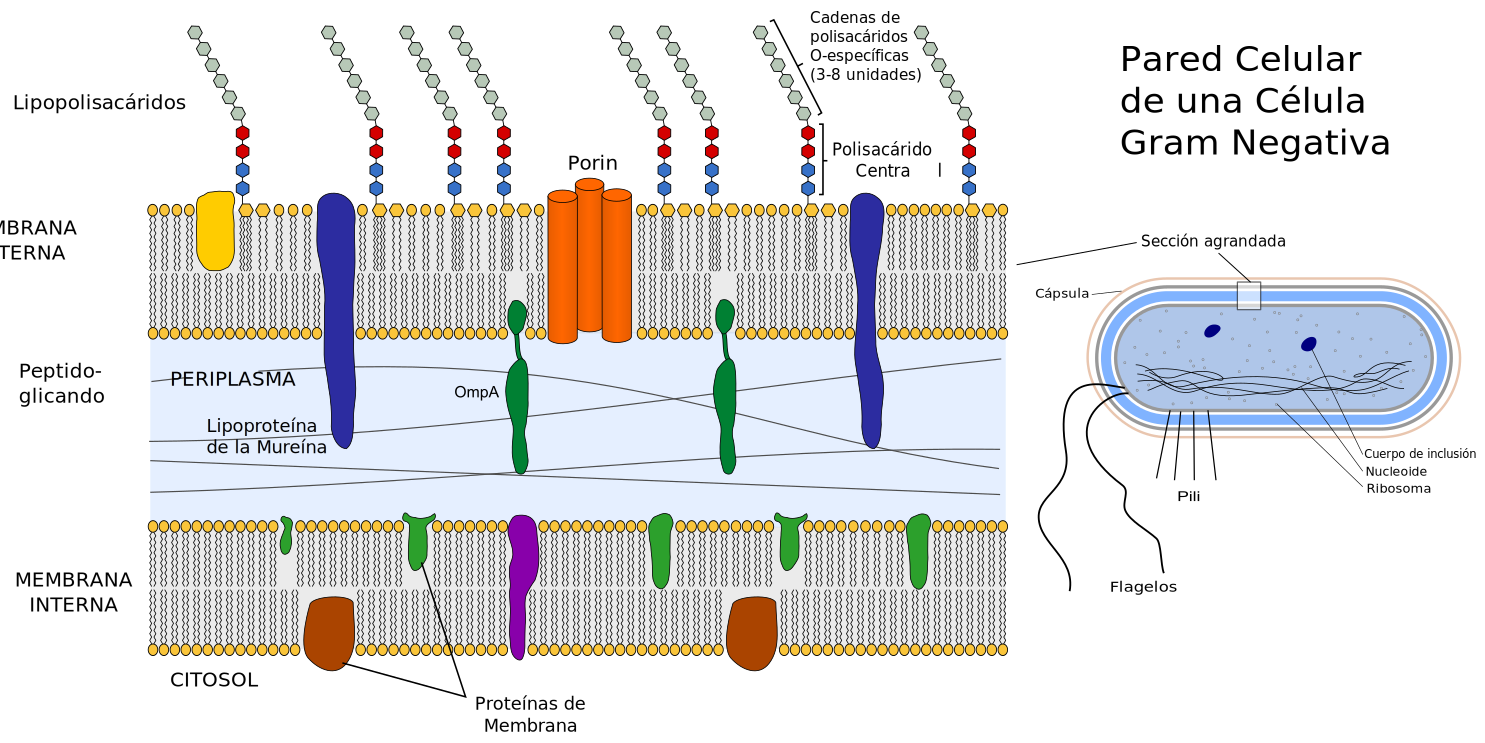
\includegraphics[scale=0.3]{Kap3/cell_wall.pdf}
\caption{Membranas interna y externa de una bacteria gram negativa mostrando algunas de las macromol\'{e}culas que la constituyen. En elmedio de las dos membranas est\'{a} la pared celular que divide el periplasma en dos partes. Traducida de \cite{Dahl2008File:Gram-}}\label{fig:cell}
\end{figure}
Tambi\'{e}n se observan macromol\'{e}culas unidas a cada membrana, algunas de estas son prote\'{i}nas de membrana. Hay prote\'{i}nas de membrana que atraviesan la membrana (prote\'{i}nas integrales de membrana) mientras que otras s\'{o}lamente est\'{a}n ubicadas en el interior o 
el exterior de la c\'{e}lula, estas son conocidas como prote\'{i}nas de membrana perif\'{e}ricas. Incluso, algunas est\'{a}n unidas con grupos no proteicos, tales como carbohidratos y l\'{i}pidos.\\

Para visualizar las membranas se puede usar el microscopio de fuerza at\'{o}mico, que muestra el perfil de la membrana con sus componenentes.\\
\subsection{Transportadores}
La membrana celular al ser hidrof\'{o}bica permite protegerse de la regi\'{o}n extracelular, sin embargo, ella necesita ingresar y expulsar todos los compuestos necesarios para realizar sus procesos metab\'{o}licos. Seg\'{u}n el tama\~{n}o, la concentraci\'{o}n y las cargas relativas de estos compuestos, estos pueden pasar directamente por la membrana lip\'{i}dica, mientras que otras requieren de las prote\'{i}nas de membrana para poder pasar al interior y/o al exterior de la c\'{e}lula. Ah\'{i} entran en juego los \textit{transportadores}, los cuales son prote\'{i}nas integrales de membrana que permiten el ingreso de sustancias al interior y al exterior de las membranas biol\'{o}gicas.\\


Algunas sustancias que pasan directamente por la bicapa fosfolp\'{i}dica son el \ce{O_2} y el \ce{CO_2} que son sustancias peque\~{n}as y apolares, estas pueden pasar por difusi\'{o}n simple, lo cual no requiere un gasto de energ\'{i}a, ya que esto es un efecto dependiente de la organizaci\'{o}n de las moleculas en el espacio, es decir, de los cambios de sus concentraciones en el espacio.\\

Los transportadores se clasifican, de acuerdo al sistema de clasificaci\'{o}n de transportadores \cite{Nelson2011}, en dos categor\'{i}as principales de las cuales se desprenden otras subcategor\'{i}as :
\begin{enumerate}
 \item \textbf{Transportadores}:
 \begin{enumerate}
 \item[1.] Transportadores activos primarios: Son aqu\'{e}llos que requieren un gasto de energ\'{i}a libre para poder mover solutos en contra de su gradiente de concentraci\'{o}n. La forma m\'{a}s conocida para proporcionar energ\'{i}a es mediante la desfosforilaci\'{o}n del ATP.
 \item[2.a] Transportadores activos secundarios (Cotransportadores \cite{Nelson2011}): Son aqu\'{e}llos que est\'{a}n mediados en los que hay un acoplamiento de dos solutos. Mientras uno es transportado a favor del gradiente de concentraci\'{o}n \footnote{Por convenci\'{o}n a favor del gradiente de concentraci\'{o}n significa que pasa de mayor a menor concentraci\'{o}n, es decir, en la direcci\'{o}n contraria al gradiente ``matem\'{a}tico'' $\nabla c$}, proporcionando energ\'{i}a libre, el otro aprovecha esta energ\'{i}a para ir en contra del gradiente de concentraci\'{o}n. Frecuentemente este proceso est\'{a} acompa\~{n}ado de un transporte activo primario, para producir el gradiente favorable de concentraci\'{o}n. Existen dos tipos:
  \begin{enumerate}
 \item[a)] Simportadores: Son los que transportan las dos sustancias en la misma direcci\'{o}n.
 \item[b)] Antiportadores: Son los que transportan las dos sustancias en direcciones contrarias.
 \end{enumerate}
 \item[2.b] Uniportadores: Se da por difusi\'{o}n facilitada, esto es, la prote\'{i}na facilita la difusi\'{o}n a favor del gradiente de concentraci\'{o}n, se presenta debido a que algunas sustancias no son solubles en l\'{i}pidos (iones o sustancias polares) o su tama\~{n}o molecular no les permite pasar.
 \end{enumerate}
 \item  \textbf{Canales i\'{o}nicos}: Los canales se diferencian de los portadores en que no necesitan energ\'{i}a metab\'{o}lica para transportar los iones. Adicional a esto, la raz\'{o}n a la que transportan los iones, es de $10^6$ iones/segundo  (muy alta).
 \end{enumerate}


\section{Simportadores de Sodio Soluto}
Hacia la d\'{e}cada de los a\~{n}os sesenta Robert Crane, ver \cite{Hamilton2013}, estableci\'{o} una relaci\'{o}n acoplada o de \textit{cotransporte} entre el ion de sodio y la glucosa los cuales son absorbidos por el intestino delgado. El conocimiento de este mecanismo ha permitido realizar el tratamiento de la diarrea y del c\'{o}lera mediante la rehidrataci\'{o}n oral. La hip\'{o}tesis del cotransporte ha sido numerosamente validada y ha sido una piedra angular para el entendimiento de el metabolismo de los carbohidratos, claves en la energ\'{e}tica celular. La hip\'{o}tesis del cotransporte tambi\'{e}n se ha extendido a otros organismos vivos, con la diferencia de que el acoplamiento del sodio se puede dar con cualquier otro soluto org\'{a}nico \cite{Faham2008}.\\

Ejemplos de simportadores que transportan el sodio acoplado con otros solutos son el transportador de \ce{Na^{+}/I^{-}} NIS encontrado en las c\'{e}lulas de la gl\'{a}ndula tiroidea, el transportador de  \ce{Na^{+}/Glucosa} SGLT1 encontrado en el intestino delgado (mencionado arriba) y el transportador de  \ce{Na^{+}/Glucosa} SGLT2 encontrado en la nefrona del ri\~{n}on.\\ 

Actualmente los simportadores de \ce{Na^+}-soluto, son una familia de prote\'{i}nas de membrana, denotada como SSS (en ingl\'{e}s Sodium Solute Symporter). La cual pertenece a la superfamilia APC (Por las siglas en ingl\'{e}s Amino acid-poliamine organocation superfamily) de la cual, una familia a resaltar es la NSS, que contiene el cotransportador de leucina y dos \ce{Na^+} LeuT, que posee un plegamiento similar al de los tranportadores mencionados (Com\'{u}nmente conocido como leuT fold o plegamiento de LeuT).\\
\section{Co-transportador vSGLT}\label{sec:esvSGLT}
El cotransportador de Na+/Galactosa presente en la membrana interna de la proteobacteria gram negativa \textit{Vibrio Parahaemolyticus} denotado como vSGLT, es un simportador perteneciente a la familia  SSS \cite{SaierJr.}, es decir, transporta simult\'{a}neamente sodio y galactosa.\\

La caracterizaci\'{o}n molecular del compuesto se realiz\'{o} por primera vez hacia el a\~{n}o 2000 por \cite{Turk2000}, mientras que la determinaci\'{o}n de su estructura fue posible hacia el a\~{n}o 2008 \cite{Faham2008}. Luego, en el a\~{n}o 2010 se determin\'{o} la estructura del mutante K294A (reemplazo de lisina por alanina) en la que aparecen registradas dos $\alpha$ h\'{e}lices adicionales.\\

En la caracterizaci\'{o}n de vSGLT, se encuentra reportada una  masa de 60676 Da y 543 residuos, equivalente a 3854 \'{a}tomos, sin incluir los hidr\'{o}genos. Adem\'{a}s este puede transportar como mon\'{o}mero,  aunque en su forma biol\'{o}gica aparece como d\'{i}mero. Principalmente transporta galactosa, aunque con un menor rendimiento puede transportar glucosa y fructosa, de la misma manera que lo hacen los transportadores SGLT1 Y SGLT2 \cite{SaierJr.}.\\

La estructura tridimensional de vSGLT \cite{Faham2008} se obtiene por difracci\'{o}n de rayos x con un espaciamiento de Bragg entre $2.7\AA$ y $3\AA$ (mejor y peor direcci\'{o}n) y  a una temperatura de $T=100$K. Esta  resoluci\'{o}n es la dada por los rayos x emitidos de una placa de cobre y corresponde al tama\~{n}o al que se alcanzan a percibir los residuos en una prote\'{i}na con posibles errores en los rotameros de las cadenas laterales peque\~{n}as \cite{Huang2007}. Se pasaron por el difract\'{o}metro tres tipos de estructuras cristalinas \ce{P1}, \ce{P2_{1}},  \ce{P2_{1}P2_{1}P2_{1}} que corresponden a los sistemas tricl\'{i}nico, monocl\'{i}nico y ortorr\'{o}mbico \footnote{Existen 7 sistemas cristalinos, cada uno de los cuales cumple una simetr\'{i}a diferente. Cada uno de estos sistemas contiene varios tipos de redes, llamadas redes de Bravais. De acuerdo a la notaci\'{o}n de Germann-Mauguin una celda primitiva se representa con la letra P, ver \cite{VainshteinModernCrystallography}.} respectivamente.\\

En la base de datos del PDB, se encuentra la estructura de vSGLT  como un tetr\'{a}mero con el c\'{o}digo PDB 3DH4, ver figura \ref{fig:3dh4}. La estructura tetram\'{e}rica es la de la celda unitaria. Mientras que en su ensamblaje biol\'{o}gico forma un d\'{i}mero, figura \label{fig:complejo} (a).

\begin{figure}[H]
\centering
\includegraphics[scale=0.1]{Kap3/3dh4tetra.png}
\caption{Tetr\'{a}mero del cotransportador vSGLT (C\'{o}digo pdb 3dh4) como aparece cristalizado.}\label{fig:3dh4}
\end{figure}
La conformaci\'{o}n con la cual se obtuvo la estructura cristalina del simportador fue la conformaci\'{o}n hacia adentro cerrada, es decir, con la galactosa ocluida dentro del simportador tal como se muestra en la figura \ref{fig:3dh4_2}. El sitio del sodio fue determinado de acuerdo a la arquitectura central (core structure) que comparte el simportador con los simportadores que pertenecen a la superfamilia del plegamiento de LeuT, la cual es cercana al sitio Na2 de LeuT. La distancia a la que se encuentran el sodio (ion) y la galactosa (substrato) es $\sim 10 \AA$\\
\begin{figure}[H]
\centering
\includegraphics[scale=0.2]{Kap3/vSGLT_in1.png}
\put(-40,0){(a)}
%\includegraphics[scale=0.07]{Kap3/vSGLT_in2.png}
%\put(-40,0){(b)}
%\vspace{10mm}
\includegraphics[scale=0.25]{Kap3/vSGLT_inward.png}
\put(-50,70){Out}
\put(-50,-5){In}
\put(-60,0){(b)}
\caption{14 segmentos transmembranales de vSGLT con sus $\alpha$ h\'{e}lices representadas por cilindros. La galactosa se muestra  ocluida.(a) Vista desde el periplasma; %(b) vista desde el citoplasma; (c)
(b) vista lateral. Figura tomada de \cite{Faham2008}}\label{fig:3dh4_2}
\end{figure}
El n\'{u}mero de segmentos transmembranales TM es de 14, los cuales est\'{a}n formados por una o a lo sumo dos $\alpha$ h\'{e}lices unidas por lazos. Los segmentos TM est\'{a}n distribuidos entre los residuos \cite{Lomize2012OPMMembranes}:\\

TM1(4-18), TM2(53-77), TM3(82-99), TM4(129-155), TM5(162-177), TM6(188-205), TM7(255-267), TM8(286-305), TM9(348-377), TM10(397-418), TM11(423-443), TM12(458-472), TM13(479-496), TM14(524-545).\\

Debe tenerse en cuenta que el TM2 est\'{a} fragmentado en dos partes:  TM2E(53-64), TM2I(67-77).\\

Posteriormente en \cite{Watanabe2010} aparece una nueva estructura del cotransportador vSGLT mutada en la posici\'{o}n K294A. Esta estructura aparece en su conformaci\'{o}n hacia adentro pero abierta o no ocluida, es decir, con el sustrato liberado. En la base de datos del PDB se encuentra reposada dicha estructura con el c\'{o}digo 2XQ2. Esta estructura difiere de 3DH4 en que all\'{i} se resuelve el segmento TM1, que aunque en la figura \ref{fig:3dh4_2} aparece como una h\'{e}lice, en esta no se conocen las posiciones de los residuos. Adicionalmente, se encuentra una he\'{e}lice adicional al final de la secuencia.\\

En la figura \ref{fig:2xq2} se muestra la unidad asim\'{e}trica (celda unitaria) obtenida por cristalograf\'{i}a de rayos x a una resoluci\'{o}n de $2.73\AA$. La unidad asim\'{e}trica est\'{a} formada por un d\'{i}mero del vSGLT. Cada mon\'{o}mero tiene 15 segmentos transmembranales.\\
\begin{figure}[H]
\centering
\includegraphics[scale=0.2]{Kap3/2xq2.png}
\caption{Unidad asim\'{e}trica del mutante K294A del cotransportador vSGLT mostrando la cadana principal en forma de "cartoon" }\label{fig:2xq2}
\end{figure}
\section{Estudios computacionales del Co-transportador vSGLT}
La estructura del mutante K294A, junto con una nueva caracterizaci\'{o}n bioqu\'{i}mica y simulaciones por din\'{a}mica molecular, todas encontradas en \cite{Watanabe2010} muestran que cuando sale el sodio, la h\'{e}lice 2 (tomada para ellos como 1) se reorienta, permitiendo que se abra la compuerta para que salga posteriormente la galactosa. Al realizar las simulaciones por din\'{a}mica molecular se encuentra que a los $\sim 52$ns la Tyr263 hace su transici\'{o}n entre dos rot\'{a}meros para dejar pasar la galactosa al espacio intracelular,  tal como se muestra en la figura \ref{fig:Y263}.\\
\begin{figure}[ht]
\centering%
\includegraphics[scale=0.4]{Kap3/Y263.png}%
\caption{Abertura de la compuerta Tyr263 para dejar la galactosa en el citoplasma.Tomada de \cite{Watanabe2010}} \label{fig:Y263}
\end{figure}
Posteriormente \cite{Adelman2016}, v\'{i}a simulaciones de din\'{a}mica molecular  encontraron que no existe no existe un orden espec\'{i}fico en que salgan el sodio y la galactosa.